\documentclass[twoside]{book}

% Packages required by doxygen
\usepackage{fixltx2e}
\usepackage{calc}
\usepackage{doxygen}
\usepackage[export]{adjustbox} % also loads graphicx
\usepackage{graphicx}
\usepackage[utf8]{inputenc}
\usepackage{makeidx}
\usepackage{multicol}
\usepackage{multirow}
\PassOptionsToPackage{warn}{textcomp}
\usepackage{textcomp}
\usepackage[nointegrals]{wasysym}
\usepackage[table]{xcolor}

% Font selection
\usepackage[T1]{fontenc}
\usepackage[scaled=.90]{helvet}
\usepackage{courier}
\usepackage{amssymb}
\usepackage{sectsty}
\renewcommand{\familydefault}{\sfdefault}
\allsectionsfont{%
  \fontseries{bc}\selectfont%
  \color{darkgray}%
}
\renewcommand{\DoxyLabelFont}{%
  \fontseries{bc}\selectfont%
  \color{darkgray}%
}
\newcommand{\+}{\discretionary{\mbox{\scriptsize$\hookleftarrow$}}{}{}}

% Page & text layout
\usepackage{geometry}
\geometry{%
  a4paper,%
  top=2.5cm,%
  bottom=2.5cm,%
  left=2.5cm,%
  right=2.5cm%
}
\tolerance=750
\hfuzz=15pt
\hbadness=750
\setlength{\emergencystretch}{15pt}
\setlength{\parindent}{0cm}
\setlength{\parskip}{3ex plus 2ex minus 2ex}
\makeatletter
\renewcommand{\paragraph}{%
  \@startsection{paragraph}{4}{0ex}{-1.0ex}{1.0ex}{%
    \normalfont\normalsize\bfseries\SS@parafont%
  }%
}
\renewcommand{\subparagraph}{%
  \@startsection{subparagraph}{5}{0ex}{-1.0ex}{1.0ex}{%
    \normalfont\normalsize\bfseries\SS@subparafont%
  }%
}
\makeatother

% Headers & footers
\usepackage{fancyhdr}
\pagestyle{fancyplain}
\fancyhead[LE]{\fancyplain{}{\bfseries\thepage}}
\fancyhead[CE]{\fancyplain{}{}}
\fancyhead[RE]{\fancyplain{}{\bfseries\leftmark}}
\fancyhead[LO]{\fancyplain{}{\bfseries\rightmark}}
\fancyhead[CO]{\fancyplain{}{}}
\fancyhead[RO]{\fancyplain{}{\bfseries\thepage}}
\fancyfoot[LE]{\fancyplain{}{}}
\fancyfoot[CE]{\fancyplain{}{}}
\fancyfoot[RE]{\fancyplain{}{\bfseries\scriptsize Generated by Doxygen }}
\fancyfoot[LO]{\fancyplain{}{\bfseries\scriptsize Generated by Doxygen }}
\fancyfoot[CO]{\fancyplain{}{}}
\fancyfoot[RO]{\fancyplain{}{}}
\renewcommand{\footrulewidth}{0.4pt}
\renewcommand{\chaptermark}[1]{%
  \markboth{#1}{}%
}
\renewcommand{\sectionmark}[1]{%
  \markright{\thesection\ #1}%
}

% Indices & bibliography
\usepackage{natbib}
\usepackage[titles]{tocloft}
\setcounter{tocdepth}{3}
\setcounter{secnumdepth}{5}
\makeindex

% Hyperlinks (required, but should be loaded last)
\usepackage{ifpdf}
\ifpdf
  \usepackage[pdftex,pagebackref=true]{hyperref}
\else
  \usepackage[ps2pdf,pagebackref=true]{hyperref}
\fi
\hypersetup{%
  colorlinks=true,%
  linkcolor=blue,%
  citecolor=blue,%
  unicode%
}

% Custom commands
\newcommand{\clearemptydoublepage}{%
  \newpage{\pagestyle{empty}\cleardoublepage}%
}

\usepackage{caption}
\captionsetup{labelsep=space,justification=centering,font={bf},singlelinecheck=off,skip=4pt,position=top}

%===== C O N T E N T S =====

\begin{document}

% Titlepage & ToC
\hypersetup{pageanchor=false,
             bookmarksnumbered=true,
             pdfencoding=unicode
            }
\pagenumbering{roman}
\begin{titlepage}
\vspace*{7cm}
\begin{center}%
{\Large R\+E\+MS Eye In Hand Registration }\\
\vspace*{1cm}
{\large Generated by Doxygen 1.8.11}\\
\end{center}
\end{titlepage}
\clearemptydoublepage
\tableofcontents
\clearemptydoublepage
\pagenumbering{arabic}
\hypersetup{pageanchor=true}

%--- Begin generated contents ---
\chapter{Hierarchical Index}
\section{Class Hierarchy}
This inheritance list is sorted roughly, but not completely, alphabetically\+:\begin{DoxyCompactList}
\item \contentsline{section}{Cloud\+Processing}{\pageref{class_cloud_processing}}{}
\item \contentsline{section}{Hand\+Eye\+Registration}{\pageref{class_hand_eye_registration}}{}
\item Handler\begin{DoxyCompactList}
\item \contentsline{section}{Camera}{\pageref{class_camera}}{}
\end{DoxyCompactList}
\item \contentsline{section}{H\+E\+Calibration}{\pageref{class_h_e_calibration}}{}
\item \contentsline{section}{Interface}{\pageref{class_interface}}{}
\end{DoxyCompactList}

\chapter{Class Index}
\section{Class List}
Here are the classes, structs, unions and interfaces with brief descriptions\+:\begin{DoxyCompactList}
\item\contentsline{section}{\hyperlink{class_camera}{Camera} \\*Manages the interface with the Intel Real Sense \hyperlink{class_camera}{Camera} }{\pageref{class_camera}}{}
\item\contentsline{section}{\hyperlink{class_cloud_processing}{Cloud\+Processing} \\*Handles the processing of point clouds. All functions are static and the class has no member variables }{\pageref{class_cloud_processing}}{}
\item\contentsline{section}{\hyperlink{class_hand_eye_registration}{Hand\+Eye\+Registration} \\*Class for computing registration between point cloud and mesh }{\pageref{class_hand_eye_registration}}{}
\item\contentsline{section}{\hyperlink{class_h_e_calibration}{H\+E\+Calibration} \\*Class that aids in performing an Eye in Hand calibration using an Angle Bracket as the calibration object. Only static methods are implemented at the moment }{\pageref{class_h_e_calibration}}{}
\item\contentsline{section}{\hyperlink{class_interface}{Interface} \\*Driver class for the R\+E\+MS Eye in Hand Registration Package }{\pageref{class_interface}}{}
\end{DoxyCompactList}

\chapter{Class Documentation}
\hypertarget{class_camera}{}\section{Camera Class Reference}
\label{class_camera}\index{Camera@{Camera}}


Manages the interface with the Intel Real Sense \hyperlink{class_camera}{Camera}.  




{\ttfamily \#include $<$Camera.\+h$>$}

Inheritance diagram for Camera\+:\begin{figure}[H]
\begin{center}
\leavevmode
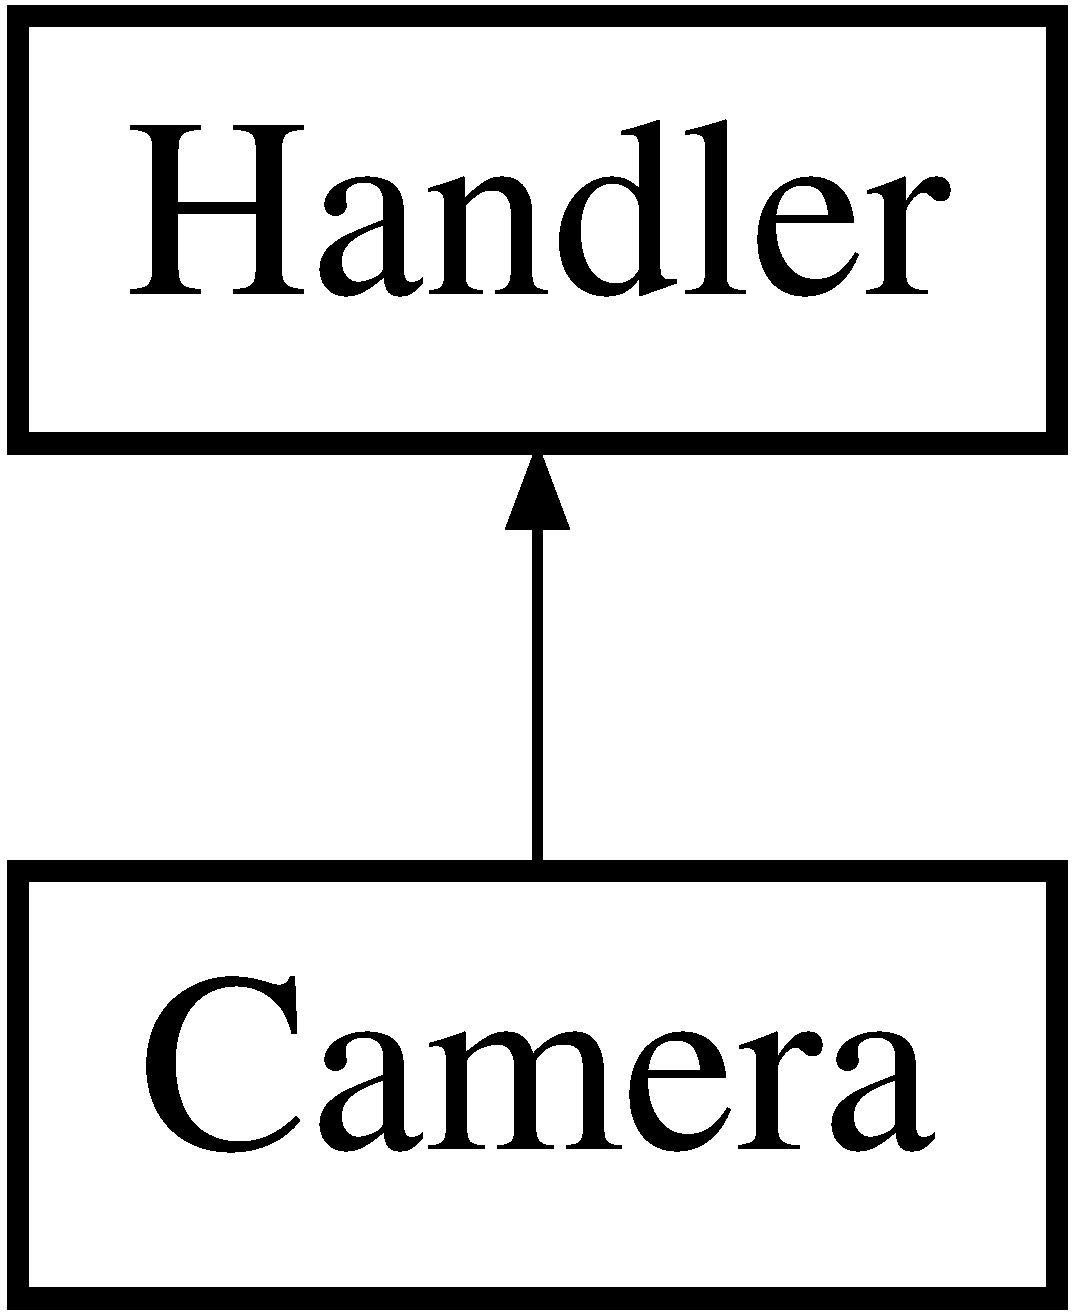
\includegraphics[height=2.000000cm]{class_camera}
\end{center}
\end{figure}
\subsection*{Public Types}
\begin{DoxyCompactItemize}
\item 
enum \hyperlink{class_camera_a83ca54501c968dae469459fb0ad78c54}{S\+Y\+N\+C\+\_\+\+O\+P\+T\+I\+ON} \{ {\bfseries S\+Y\+N\+C\+\_\+\+O\+P\+T\+I\+O\+N\+\_\+\+SW} = 0, 
{\bfseries S\+Y\+N\+C\+\_\+\+O\+P\+T\+I\+O\+N\+\_\+\+HW}, 
{\bfseries S\+Y\+N\+C\+\_\+\+O\+P\+T\+I\+O\+N\+\_\+\+N\+O\+NE}
 \}
\end{DoxyCompactItemize}
\subsection*{Public Member Functions}
\begin{DoxyCompactItemize}
\item 
\hyperlink{class_camera_a01f94c3543f56ede7af49dc778f19331}{Camera} ()
\item 
void \hyperlink{class_camera_aec22c94e7bcc461154085ef31c5de125}{get\+Frame} (vct\+Dynamic\+Vector$<$ vct3 $>$ \&points)
\end{DoxyCompactItemize}
\subsection*{Protected Attributes}
\begin{DoxyCompactItemize}
\item 
P\+X\+C\+Sense\+Manager $\ast$ {\bfseries sm}\hypertarget{class_camera_aac4ebf35b8a29c3c233a12f1e6294292}{}\label{class_camera_aac4ebf35b8a29c3c233a12f1e6294292}

\end{DoxyCompactItemize}


\subsection{Detailed Description}
Manages the interface with the Intel Real Sense \hyperlink{class_camera}{Camera}. 

This class uses the windows R\+S\+S\+DK to configure and get points clouds from the camera. It streams in a resolution of 640x480 with a frame rate of 30. 

\subsection{Member Enumeration Documentation}
\index{Camera@{Camera}!S\+Y\+N\+C\+\_\+\+O\+P\+T\+I\+ON@{S\+Y\+N\+C\+\_\+\+O\+P\+T\+I\+ON}}
\index{S\+Y\+N\+C\+\_\+\+O\+P\+T\+I\+ON@{S\+Y\+N\+C\+\_\+\+O\+P\+T\+I\+ON}!Camera@{Camera}}
\subsubsection[{\texorpdfstring{S\+Y\+N\+C\+\_\+\+O\+P\+T\+I\+ON}{SYNC_OPTION}}]{\setlength{\rightskip}{0pt plus 5cm}enum {\bf Camera\+::\+S\+Y\+N\+C\+\_\+\+O\+P\+T\+I\+ON}}\hypertarget{class_camera_a83ca54501c968dae469459fb0ad78c54}{}\label{class_camera_a83ca54501c968dae469459fb0ad78c54}
Enum for how the sync the streams. 

\subsection{Constructor \& Destructor Documentation}
\index{Camera@{Camera}!Camera@{Camera}}
\index{Camera@{Camera}!Camera@{Camera}}
\subsubsection[{\texorpdfstring{Camera()}{Camera()}}]{\setlength{\rightskip}{0pt plus 5cm}Camera\+::\+Camera (
\begin{DoxyParamCaption}
{}
\end{DoxyParamCaption}
)}\hypertarget{class_camera_a01f94c3543f56ede7af49dc778f19331}{}\label{class_camera_a01f94c3543f56ede7af49dc778f19331}
Basic constructor. Doesn\textquotesingle{}t do anything. All initialization occurs when \hyperlink{class_camera_aec22c94e7bcc461154085ef31c5de125}{get\+Frame()} is called to ensure that changes in camera in between calls don\textquotesingle{}t cause problems. 

\subsection{Member Function Documentation}
\index{Camera@{Camera}!get\+Frame@{get\+Frame}}
\index{get\+Frame@{get\+Frame}!Camera@{Camera}}
\subsubsection[{\texorpdfstring{get\+Frame(vct\+Dynamic\+Vector$<$ vct3 $>$ \&points)}{getFrame(vctDynamicVector< vct3 > &points)}}]{\setlength{\rightskip}{0pt plus 5cm}void Camera\+::get\+Frame (
\begin{DoxyParamCaption}
\item[{vct\+Dynamic\+Vector$<$ vct3 $>$ \&}]{points}
\end{DoxyParamCaption}
)}\hypertarget{class_camera_aec22c94e7bcc461154085ef31c5de125}{}\label{class_camera_aec22c94e7bcc461154085ef31c5de125}
Gets a point cloud from the camera and loads it into the array. This is done using the P\+X\+C\+Projection mapping, which maps the pixelX, pixelY, depth points to x,y,z vertices. 
\begin{DoxyParams}[1]{Parameters}
\mbox{\tt out}  & {\em points} & The vector of points to load the point cloud into \\
\hline
\end{DoxyParams}


The documentation for this class was generated from the following files\+:\begin{DoxyCompactItemize}
\item 
Camera.\+h\item 
Camera.\+cpp\end{DoxyCompactItemize}

\hypertarget{class_cloud_processing}{}\section{Cloud\+Processing Class Reference}
\label{class_cloud_processing}\index{Cloud\+Processing@{Cloud\+Processing}}


Handles the processing of point clouds. All functions are static and the class has no member variables.  




{\ttfamily \#include $<$Cloud\+Processing.\+h$>$}

\subsection*{Static Public Member Functions}
\begin{DoxyCompactItemize}
\item 
static void \hyperlink{class_cloud_processing_aef2ec63d577ce493f24c69e2a6d68ca7}{T\+X\+Tto\+P\+CD} (std\+::string filename)
\item 
static void \hyperlink{class_cloud_processing_a8a3e98139d08714e346ccfe0d8cbb240}{view\+Clouds\+From\+Files} (std\+::vector$<$ std\+::string $>$ filenames)
\item 
static vct\+Dynamic\+Vector$<$ vct3 $>$ \hyperlink{class_cloud_processing_a87725c89d18cdb9f31ecd5ccbe3daf87}{P\+C\+Lto\+C\+I\+S\+ST} (pcl\+::\+Point\+Cloud$<$ pcl\+::\+Point\+X\+YZ $>$\+::Ptr cloud)
\item 
static pcl\+::\+Point\+Cloud$<$ pcl\+::\+Point\+X\+YZ $>$\+::Ptr \hyperlink{class_cloud_processing_a8236eb8ff46125992a136661ca26051d}{C\+I\+S\+S\+Tto\+P\+CL} (vct\+Dynamic\+Vector$<$ vct3 $>$ points)
\item 
static void \hyperlink{class_cloud_processing_aed3aed29847bc8eaca0e68994abf7f01}{view\+Clouds} (std\+::vector$<$ pcl\+::\+Point\+Cloud$<$ pcl\+::\+Point\+X\+YZ $>$ $>$ $\ast$clouds)
\item 
static pcl\+::\+Point\+Cloud$<$ pcl\+::\+Point\+X\+YZ $>$\+::Ptr \hyperlink{class_cloud_processing_ae58e471bf180c4ddda64c02f69fee331}{downsample\+\_\+cloud} (pcl\+::\+Point\+Cloud$<$ pcl\+::\+Point\+X\+YZ $>$\+::Ptr cloud, float leaf\+\_\+size)
\item 
static pcl\+::\+Point\+Cloud$<$ pcl\+::\+Point\+X\+YZ $>$\+::Ptr \hyperlink{class_cloud_processing_a41c6b9aa981bd642f22d4272a2dc7666}{remove\+\_\+plane} (pcl\+::\+Point\+Cloud$<$ pcl\+::\+Point\+X\+YZ $>$\+::Ptr cloud, float tolerance)
\end{DoxyCompactItemize}


\subsection{Detailed Description}
Handles the processing of point clouds. All functions are static and the class has no member variables. 

This class handles all interfacing with P\+CL and manages the visualization, downsampling, and segmentation of point clouds. All methods are static. 

\subsection{Member Function Documentation}
\index{Cloud\+Processing@{Cloud\+Processing}!C\+I\+S\+S\+Tto\+P\+CL@{C\+I\+S\+S\+Tto\+P\+CL}}
\index{C\+I\+S\+S\+Tto\+P\+CL@{C\+I\+S\+S\+Tto\+P\+CL}!Cloud\+Processing@{Cloud\+Processing}}
\subsubsection[{\texorpdfstring{C\+I\+S\+S\+Tto\+P\+C\+L(vct\+Dynamic\+Vector$<$ vct3 $>$ points)}{CISSTtoPCL(vctDynamicVector< vct3 > points)}}]{\setlength{\rightskip}{0pt plus 5cm}pcl\+::\+Point\+Cloud$<$ pcl\+::\+Point\+X\+YZ $>$\+::Ptr Cloud\+Processing\+::\+C\+I\+S\+S\+Tto\+P\+CL (
\begin{DoxyParamCaption}
\item[{vct\+Dynamic\+Vector$<$ vct3 $>$}]{points}
\end{DoxyParamCaption}
)\hspace{0.3cm}{\ttfamily [static]}}\hypertarget{class_cloud_processing_a8236eb8ff46125992a136661ca26051d}{}\label{class_cloud_processing_a8236eb8ff46125992a136661ca26051d}
Does the inverse function as P\+C\+Lto\+C\+I\+S\+ST 
\begin{DoxyParams}[1]{Parameters}
\mbox{\tt in}  & {\em points} & the list of points to be converted into a P\+CL cloud \\
\hline
\end{DoxyParams}
\begin{DoxyReturn}{Returns}
Returns a boost managed ptr to the cloud, which now stores the points that were passed in with the vct\+Dynamic\+Vector 
\end{DoxyReturn}
\index{Cloud\+Processing@{Cloud\+Processing}!downsample\+\_\+cloud@{downsample\+\_\+cloud}}
\index{downsample\+\_\+cloud@{downsample\+\_\+cloud}!Cloud\+Processing@{Cloud\+Processing}}
\subsubsection[{\texorpdfstring{downsample\+\_\+cloud(pcl\+::\+Point\+Cloud$<$ pcl\+::\+Point\+X\+Y\+Z $>$\+::\+Ptr cloud, float leaf\+\_\+size)}{downsample_cloud(pcl::PointCloud< pcl::PointXYZ >::Ptr cloud, float leaf_size)}}]{\setlength{\rightskip}{0pt plus 5cm}pcl\+::\+Point\+Cloud$<$ pcl\+::\+Point\+X\+YZ $>$\+::Ptr Cloud\+Processing\+::downsample\+\_\+cloud (
\begin{DoxyParamCaption}
\item[{pcl\+::\+Point\+Cloud$<$ pcl\+::\+Point\+X\+YZ $>$\+::Ptr}]{cloud, }
\item[{float}]{leaf\+\_\+size}
\end{DoxyParamCaption}
)\hspace{0.3cm}{\ttfamily [static]}}\hypertarget{class_cloud_processing_ae58e471bf180c4ddda64c02f69fee331}{}\label{class_cloud_processing_ae58e471bf180c4ddda64c02f69fee331}
This function downsamples the given point cloud by constructing a KD tree where the dimensions of the bounding box of each leaf node is leaf\+\_\+size. It then makes a new cloud where the points are the centroids of all the leaf nodes from the KD tree. 
\begin{DoxyParams}[1]{Parameters}
\mbox{\tt in}  & {\em cloud} & The cloud to downsample \mbox{[}in\mbox{]} The size of the bounding box for the leaf\+\_\+nodes. Units are millimetres \\
\hline
\end{DoxyParams}
\begin{DoxyReturn}{Returns}
A new cloud that is the \char`\"{}downsampled\char`\"{} version of the original 
\end{DoxyReturn}
\index{Cloud\+Processing@{Cloud\+Processing}!P\+C\+Lto\+C\+I\+S\+ST@{P\+C\+Lto\+C\+I\+S\+ST}}
\index{P\+C\+Lto\+C\+I\+S\+ST@{P\+C\+Lto\+C\+I\+S\+ST}!Cloud\+Processing@{Cloud\+Processing}}
\subsubsection[{\texorpdfstring{P\+C\+Lto\+C\+I\+S\+S\+T(pcl\+::\+Point\+Cloud$<$ pcl\+::\+Point\+X\+Y\+Z $>$\+::\+Ptr cloud)}{PCLtoCISST(pcl::PointCloud< pcl::PointXYZ >::Ptr cloud)}}]{\setlength{\rightskip}{0pt plus 5cm}vct\+Dynamic\+Vector$<$ vct3 $>$ Cloud\+Processing\+::\+P\+C\+Lto\+C\+I\+S\+ST (
\begin{DoxyParamCaption}
\item[{pcl\+::\+Point\+Cloud$<$ pcl\+::\+Point\+X\+YZ $>$\+::Ptr}]{cloud}
\end{DoxyParamCaption}
)\hspace{0.3cm}{\ttfamily [static]}}\hypertarget{class_cloud_processing_a87725c89d18cdb9f31ecd5ccbe3daf87}{}\label{class_cloud_processing_a87725c89d18cdb9f31ecd5ccbe3daf87}
Converts a point cloud from the P\+CL format to be stored as vct\+Dynamic\+Vector$<$vct3$>$ list of points. 
\begin{DoxyParams}[1]{Parameters}
\mbox{\tt in}  & {\em cloud} & A boost managed ptr to the point cloud to be converted \\
\hline
\end{DoxyParams}
\begin{DoxyReturn}{Returns}
This function returns the list of points that the cloud contained, but stored as vct\+Dynamic\+Vector$<$vct3$>$ 
\end{DoxyReturn}
\index{Cloud\+Processing@{Cloud\+Processing}!remove\+\_\+plane@{remove\+\_\+plane}}
\index{remove\+\_\+plane@{remove\+\_\+plane}!Cloud\+Processing@{Cloud\+Processing}}
\subsubsection[{\texorpdfstring{remove\+\_\+plane(pcl\+::\+Point\+Cloud$<$ pcl\+::\+Point\+X\+Y\+Z $>$\+::\+Ptr cloud, float tolerance)}{remove_plane(pcl::PointCloud< pcl::PointXYZ >::Ptr cloud, float tolerance)}}]{\setlength{\rightskip}{0pt plus 5cm}pcl\+::\+Point\+Cloud$<$ pcl\+::\+Point\+X\+YZ $>$\+::Ptr Cloud\+Processing\+::remove\+\_\+plane (
\begin{DoxyParamCaption}
\item[{pcl\+::\+Point\+Cloud$<$ pcl\+::\+Point\+X\+YZ $>$\+::Ptr}]{cloud, }
\item[{float}]{tolerance}
\end{DoxyParamCaption}
)\hspace{0.3cm}{\ttfamily [static]}}\hypertarget{class_cloud_processing_a41c6b9aa981bd642f22d4272a2dc7666}{}\label{class_cloud_processing_a41c6b9aa981bd642f22d4272a2dc7666}
Removes a plane from the given cloud using the R\+A\+N\+S\+AC algorithm and P\+CL\textquotesingle{}s S\+A\+C\+Segmentation function. 
\begin{DoxyParams}[1]{Parameters}
\mbox{\tt in}  & {\em cloud} & The point cloud that has the plane to be removed \\
\hline
\mbox{\tt in}  & {\em tolerance} & The tolerance for the plane. In other words points that lie within \char`\"{}tolerance\char`\"{} of the computed plane will be removed from the cloud. Unit is mm \\
\hline
\end{DoxyParams}
\begin{DoxyReturn}{Returns}
The new cloud with the plane removed 
\end{DoxyReturn}
\index{Cloud\+Processing@{Cloud\+Processing}!T\+X\+Tto\+P\+CD@{T\+X\+Tto\+P\+CD}}
\index{T\+X\+Tto\+P\+CD@{T\+X\+Tto\+P\+CD}!Cloud\+Processing@{Cloud\+Processing}}
\subsubsection[{\texorpdfstring{T\+X\+Tto\+P\+C\+D(std\+::string filename)}{TXTtoPCD(std::string filename)}}]{\setlength{\rightskip}{0pt plus 5cm}void Cloud\+Processing\+::\+T\+X\+Tto\+P\+CD (
\begin{DoxyParamCaption}
\item[{std\+::string}]{filename}
\end{DoxyParamCaption}
)\hspace{0.3cm}{\ttfamily [static]}}\hypertarget{class_cloud_processing_aef2ec63d577ce493f24c69e2a6d68ca7}{}\label{class_cloud_processing_aef2ec63d577ce493f24c69e2a6d68ca7}
Converts a .txt file where the format is x y z on each line to a pcd file with the proper header. 
\begin{DoxyParams}[1]{Parameters}
\mbox{\tt in}  & {\em filename} & the name of the file relative to the working directory of the project to convert to pcd. Must be properly formatted. \\
\hline
\end{DoxyParams}
\index{Cloud\+Processing@{Cloud\+Processing}!view\+Clouds@{view\+Clouds}}
\index{view\+Clouds@{view\+Clouds}!Cloud\+Processing@{Cloud\+Processing}}
\subsubsection[{\texorpdfstring{view\+Clouds(std\+::vector$<$ pcl\+::\+Point\+Cloud$<$ pcl\+::\+Point\+X\+Y\+Z $>$ $>$ $\ast$clouds)}{viewClouds(std::vector< pcl::PointCloud< pcl::PointXYZ > > *clouds)}}]{\setlength{\rightskip}{0pt plus 5cm}void Cloud\+Processing\+::view\+Clouds (
\begin{DoxyParamCaption}
\item[{std\+::vector$<$ pcl\+::\+Point\+Cloud$<$ pcl\+::\+Point\+X\+YZ $>$ $>$ $\ast$}]{clouds}
\end{DoxyParamCaption}
)\hspace{0.3cm}{\ttfamily [static]}}\hypertarget{class_cloud_processing_aed3aed29847bc8eaca0e68994abf7f01}{}\label{class_cloud_processing_aed3aed29847bc8eaca0e68994abf7f01}
Visualizes an array of clouds. 
\begin{DoxyParams}[1]{Parameters}
\mbox{\tt in}  & {\em clouds} & A pointer to the vector of clouds to be visualized. \\
\hline
\end{DoxyParams}
\index{Cloud\+Processing@{Cloud\+Processing}!view\+Clouds\+From\+Files@{view\+Clouds\+From\+Files}}
\index{view\+Clouds\+From\+Files@{view\+Clouds\+From\+Files}!Cloud\+Processing@{Cloud\+Processing}}
\subsubsection[{\texorpdfstring{view\+Clouds\+From\+Files(std\+::vector$<$ std\+::string $>$ filenames)}{viewCloudsFromFiles(std::vector< std::string > filenames)}}]{\setlength{\rightskip}{0pt plus 5cm}void Cloud\+Processing\+::view\+Clouds\+From\+Files (
\begin{DoxyParamCaption}
\item[{std\+::vector$<$ std\+::string $>$}]{filenames}
\end{DoxyParamCaption}
)\hspace{0.3cm}{\ttfamily [static]}}\hypertarget{class_cloud_processing_a8a3e98139d08714e346ccfe0d8cbb240}{}\label{class_cloud_processing_a8a3e98139d08714e346ccfe0d8cbb240}
Visualizes clouds read in from files. Files must be properly formatted P\+CD files. There is no set limit on the number of files but the visualizer can only handle so many. 
\begin{DoxyParams}[1]{Parameters}
\mbox{\tt in}  & {\em filenames} & the list of filenames relative to the working directory to read the point clouds from \\
\hline
\end{DoxyParams}


The documentation for this class was generated from the following files\+:\begin{DoxyCompactItemize}
\item 
Cloud\+Processing.\+h\item 
Cloud\+Processing.\+cpp\end{DoxyCompactItemize}

\hypertarget{class_hand_eye_registration}{}\section{Hand\+Eye\+Registration Class Reference}
\label{class_hand_eye_registration}\index{Hand\+Eye\+Registration@{Hand\+Eye\+Registration}}


Class for computing registration between point cloud and mesh.  




{\ttfamily \#include $<$Registration.\+h$>$}

\subsection*{Public Member Functions}
\begin{DoxyCompactItemize}
\item 
void \hyperlink{class_hand_eye_registration_a9734ab868be5a34a95a5790f44808d1b}{load\+Mesh} (std\+::string filename)
\item 
vct\+Frm3 \hyperlink{class_hand_eye_registration_a311fe0a35cdc698e68e26d7b742bb21f}{compute\+Transform} (vct\+Dynamic\+Vector$<$ vct3 $>$ \&points)
\end{DoxyCompactItemize}
\subsection*{Static Public Member Functions}
\begin{DoxyCompactItemize}
\item 
static void \hyperlink{class_hand_eye_registration_aacb8a8fe65f148fc7b3ed77e9a6948a1}{Callback\+\_\+\+Track\+Reg\+Path} (cisst\+I\+C\+P\+::\+Callback\+Arg \&arg, void $\ast$user\+Data)
\item 
static void \hyperlink{class_hand_eye_registration_af3244e35eec3e903492458c40c8cfd0e}{Callback\+\_\+\+Save\+Iterations\+To\+File} (cisst\+I\+C\+P\+::\+Callback\+Arg \&arg, void $\ast$user\+Data)
\end{DoxyCompactItemize}


\subsection{Detailed Description}
Class for computing registration between point cloud and mesh. 

This class uses Seth Billing\textquotesingle{}s I\+CP Implementation to compute the transformation between a poin cloud and a mesh. The registration is fairly slow when run on meshes and point clouds of the sizes that CT scans and the Real Sense camera generate, so downsampling and mesh simplification are required. The registration is quite error prone and seems to often hit local minimum when computing the transformation. Further investigation into this is required, although it may simply be a result of attempting to register a partial section (since the camera can only see a section of the head) and the fact that the head is a fairly spherical object. 

\subsection{Member Function Documentation}
\index{Hand\+Eye\+Registration@{Hand\+Eye\+Registration}!Callback\+\_\+\+Save\+Iterations\+To\+File@{Callback\+\_\+\+Save\+Iterations\+To\+File}}
\index{Callback\+\_\+\+Save\+Iterations\+To\+File@{Callback\+\_\+\+Save\+Iterations\+To\+File}!Hand\+Eye\+Registration@{Hand\+Eye\+Registration}}
\subsubsection[{\texorpdfstring{Callback\+\_\+\+Save\+Iterations\+To\+File(cisst\+I\+C\+P\+::\+Callback\+Arg \&arg, void $\ast$user\+Data)}{Callback_SaveIterationsToFile(cisstICP::CallbackArg &arg, void *userData)}}]{\setlength{\rightskip}{0pt plus 5cm}void Hand\+Eye\+Registration\+::\+Callback\+\_\+\+Save\+Iterations\+To\+File (
\begin{DoxyParamCaption}
\item[{cisst\+I\+C\+P\+::\+Callback\+Arg \&}]{arg, }
\item[{void $\ast$}]{user\+Data}
\end{DoxyParamCaption}
)\hspace{0.3cm}{\ttfamily [static]}}\hypertarget{class_hand_eye_registration_af3244e35eec3e903492458c40c8cfd0e}{}\label{class_hand_eye_registration_af3244e35eec3e903492458c40c8cfd0e}
This function allows for I\+CP to output some debug information to a file \index{Hand\+Eye\+Registration@{Hand\+Eye\+Registration}!Callback\+\_\+\+Track\+Reg\+Path@{Callback\+\_\+\+Track\+Reg\+Path}}
\index{Callback\+\_\+\+Track\+Reg\+Path@{Callback\+\_\+\+Track\+Reg\+Path}!Hand\+Eye\+Registration@{Hand\+Eye\+Registration}}
\subsubsection[{\texorpdfstring{Callback\+\_\+\+Track\+Reg\+Path(cisst\+I\+C\+P\+::\+Callback\+Arg \&arg, void $\ast$user\+Data)}{Callback_TrackRegPath(cisstICP::CallbackArg &arg, void *userData)}}]{\setlength{\rightskip}{0pt plus 5cm}void Hand\+Eye\+Registration\+::\+Callback\+\_\+\+Track\+Reg\+Path (
\begin{DoxyParamCaption}
\item[{cisst\+I\+C\+P\+::\+Callback\+Arg \&}]{arg, }
\item[{void $\ast$}]{user\+Data}
\end{DoxyParamCaption}
)\hspace{0.3cm}{\ttfamily [static]}}\hypertarget{class_hand_eye_registration_aacb8a8fe65f148fc7b3ed77e9a6948a1}{}\label{class_hand_eye_registration_aacb8a8fe65f148fc7b3ed77e9a6948a1}
This function is a callback that allows for I\+CP output \index{Hand\+Eye\+Registration@{Hand\+Eye\+Registration}!compute\+Transform@{compute\+Transform}}
\index{compute\+Transform@{compute\+Transform}!Hand\+Eye\+Registration@{Hand\+Eye\+Registration}}
\subsubsection[{\texorpdfstring{compute\+Transform(vct\+Dynamic\+Vector$<$ vct3 $>$ \&points)}{computeTransform(vctDynamicVector< vct3 > &points)}}]{\setlength{\rightskip}{0pt plus 5cm}vct\+Frm3 Hand\+Eye\+Registration\+::compute\+Transform (
\begin{DoxyParamCaption}
\item[{vct\+Dynamic\+Vector$<$ vct3 $>$ \&}]{points}
\end{DoxyParamCaption}
)}\hypertarget{class_hand_eye_registration_a311fe0a35cdc698e68e26d7b742bb21f}{}\label{class_hand_eye_registration_a311fe0a35cdc698e68e26d7b742bb21f}
Computes the transform using I\+CP between the point cloud and the mesh that it has previously loaded. 
\begin{DoxyParams}{Parameters}
{\em points} & The point cloud to compute the transformation with \\
\hline
\end{DoxyParams}
\begin{DoxyReturn}{Returns}
the computed transformation 
\end{DoxyReturn}
\index{Hand\+Eye\+Registration@{Hand\+Eye\+Registration}!load\+Mesh@{load\+Mesh}}
\index{load\+Mesh@{load\+Mesh}!Hand\+Eye\+Registration@{Hand\+Eye\+Registration}}
\subsubsection[{\texorpdfstring{load\+Mesh(std\+::string filename)}{loadMesh(std::string filename)}}]{\setlength{\rightskip}{0pt plus 5cm}void Hand\+Eye\+Registration\+::load\+Mesh (
\begin{DoxyParamCaption}
\item[{std\+::string}]{filename}
\end{DoxyParamCaption}
)}\hypertarget{class_hand_eye_registration_a9734ab868be5a34a95a5790f44808d1b}{}\label{class_hand_eye_registration_a9734ab868be5a34a95a5790f44808d1b}
This function reads a mesh in from a file into a cisst\+Mesh data structure. I would have liked to have it also create the P\+D\+Tree for the mesh, but for some reason this caused memory issues and caused the program to crash. Not sure why, but it seemed like it had to do with how the P\+D\+Tree gets handled by managed ptrs. 
\begin{DoxyParams}{Parameters}
{\em filename} & The file to read the mesh in from. Must be formatted correctly. \\
\hline
\end{DoxyParams}


The documentation for this class was generated from the following files\+:\begin{DoxyCompactItemize}
\item 
Registration.\+h\item 
Registration.\+cpp\end{DoxyCompactItemize}

\hypertarget{class_h_e_calibration}{}\section{H\+E\+Calibration Class Reference}
\label{class_h_e_calibration}\index{H\+E\+Calibration@{H\+E\+Calibration}}


Class that aids in performing an Eye in Hand calibration using an Angle Bracket as the calibration object. Only static methods are implemented at the moment.  




{\ttfamily \#include $<$H\+E\+Calibration.\+h$>$}

\subsection*{Public Member Functions}
\begin{DoxyCompactItemize}
\item 
vct\+Frm3 \hyperlink{class_h_e_calibration_ab2765aa44f4e2359a67ad8e8ab61db64}{Get\+Wrist\+Camera\+Registration} ()
\item 
void \hyperlink{class_h_e_calibration_a26f30368c98903e7b75aaefb5f0f4038}{add\+Point\+Cloud} (cisst\+Point\+Cloud cloud)
\item 
void \hyperlink{class_h_e_calibration_a67724f066c95632eb50a557c9a22d5a3}{add\+Pose} (vct\+Frm3 pose)
\end{DoxyCompactItemize}
\subsection*{Static Public Member Functions}
\begin{DoxyCompactItemize}
\item 
static vct\+Frm3 \hyperlink{class_h_e_calibration_ab58622d16367aa3a095ce63e7d115e15}{read\+Object\+Pose} (std\+::string filename)
\item 
static std\+::vector$<$ vct\+Frm3 $>$ \hyperlink{class_h_e_calibration_a3142d195d52b7d0fba0e3c77c3f37c5f}{read\+Robot\+Poses} (std\+::string filename)
\item 
static vct\+Rot3 \hyperlink{class_h_e_calibration_a85aa37c2653082ffe3b6be85242d2617}{axxb} (std\+::vector$<$ vct\+Frm3 $>$ A, std\+::vector$<$ vct\+Frm3 $>$ B)
\item 
static vct\+Frm3 \hyperlink{class_h_e_calibration_a56ea97fc635496a57f33c573b33fd0af}{least\+Squares} (vct\+Rot3 Rx, std\+::vector$<$ vct\+Frm3 $>$ A, std\+::vector$<$ vct\+Frm3 $>$ B)
\end{DoxyCompactItemize}


\subsection{Detailed Description}
Class that aids in performing an Eye in Hand calibration using an Angle Bracket as the calibration object. Only static methods are implemented at the moment. 

This class is designed to preform a calibration using two sets of data. The first is a set of point clouds where each point cloud is from the Real Sense camera at a different robot pose. These point clouds should be of our calibration object, which is a large angle bracket s.\+t. there are three planes clearly visible in the point cloud (the two inside edges of the bracket and the table). However this class is not fully implemented. At the moment only the static (mathematical and file reading) methods are implemented. The processing of the point clouds to generate the poses is not yet implemented. 

\subsection{Member Function Documentation}
\index{H\+E\+Calibration@{H\+E\+Calibration}!add\+Point\+Cloud@{add\+Point\+Cloud}}
\index{add\+Point\+Cloud@{add\+Point\+Cloud}!H\+E\+Calibration@{H\+E\+Calibration}}
\subsubsection[{\texorpdfstring{add\+Point\+Cloud(cisst\+Point\+Cloud cloud)}{addPointCloud(cisstPointCloud cloud)}}]{\setlength{\rightskip}{0pt plus 5cm}void H\+E\+Calibration\+::add\+Point\+Cloud (
\begin{DoxyParamCaption}
\item[{cisst\+Point\+Cloud}]{cloud}
\end{DoxyParamCaption}
)}\hypertarget{class_h_e_calibration_a26f30368c98903e7b75aaefb5f0f4038}{}\label{class_h_e_calibration_a26f30368c98903e7b75aaefb5f0f4038}
Add a point cloud to the set of data for the calibration. Not yet implemented. 
\begin{DoxyParams}[1]{Parameters}
\mbox{\tt in}  & {\em cloud} & the point cloud to be added \\
\hline
\end{DoxyParams}
\index{H\+E\+Calibration@{H\+E\+Calibration}!add\+Pose@{add\+Pose}}
\index{add\+Pose@{add\+Pose}!H\+E\+Calibration@{H\+E\+Calibration}}
\subsubsection[{\texorpdfstring{add\+Pose(vct\+Frm3 pose)}{addPose(vctFrm3 pose)}}]{\setlength{\rightskip}{0pt plus 5cm}void H\+E\+Calibration\+::add\+Pose (
\begin{DoxyParamCaption}
\item[{vct\+Frm3}]{pose}
\end{DoxyParamCaption}
)}\hypertarget{class_h_e_calibration_a67724f066c95632eb50a557c9a22d5a3}{}\label{class_h_e_calibration_a67724f066c95632eb50a557c9a22d5a3}
Add a robot pose to the set of data for calibration. Not yet implemented. 
\begin{DoxyParams}[1]{Parameters}
\mbox{\tt in}  & {\em pose} & the pose to be used in the calibration. \\
\hline
\end{DoxyParams}
\index{H\+E\+Calibration@{H\+E\+Calibration}!axxb@{axxb}}
\index{axxb@{axxb}!H\+E\+Calibration@{H\+E\+Calibration}}
\subsubsection[{\texorpdfstring{axxb(std\+::vector$<$ vct\+Frm3 $>$ A, std\+::vector$<$ vct\+Frm3 $>$ B)}{axxb(std::vector< vctFrm3 > A, std::vector< vctFrm3 > B)}}]{\setlength{\rightskip}{0pt plus 5cm}vct\+Rot3 H\+E\+Calibration\+::axxb (
\begin{DoxyParamCaption}
\item[{std\+::vector$<$ vct\+Frm3 $>$}]{A, }
\item[{std\+::vector$<$ vct\+Frm3 $>$}]{B}
\end{DoxyParamCaption}
)\hspace{0.3cm}{\ttfamily [static]}}\hypertarget{class_h_e_calibration_a85aa37c2653082ffe3b6be85242d2617}{}\label{class_h_e_calibration_a85aa37c2653082ffe3b6be85242d2617}
Computes X that minmizes the error of AX=XB. This is done using the quaternion method as discussed in Dr. Russell Taylor\textquotesingle{}s lectures. 
\begin{DoxyParams}{Parameters}
{\em A\mbox{[}in\mbox{]}} & The set of poses representing the changes in position of the robot wrist \\
\hline
{\em B\mbox{[}in\mbox{]}} & The set of poses representing the changes in position of the calibration object relative to the camera \\
\hline
\end{DoxyParams}
\begin{DoxyReturn}{Returns}
The best solution for the rotational component of the transformation from the wrist to the camera 
\end{DoxyReturn}
\index{H\+E\+Calibration@{H\+E\+Calibration}!Get\+Wrist\+Camera\+Registration@{Get\+Wrist\+Camera\+Registration}}
\index{Get\+Wrist\+Camera\+Registration@{Get\+Wrist\+Camera\+Registration}!H\+E\+Calibration@{H\+E\+Calibration}}
\subsubsection[{\texorpdfstring{Get\+Wrist\+Camera\+Registration()}{GetWristCameraRegistration()}}]{\setlength{\rightskip}{0pt plus 5cm}vct\+Frm3 H\+E\+Calibration\+::\+Get\+Wrist\+Camera\+Registration (
\begin{DoxyParamCaption}
{}
\end{DoxyParamCaption}
)}\hypertarget{class_h_e_calibration_ab2765aa44f4e2359a67ad8e8ab61db64}{}\label{class_h_e_calibration_ab2765aa44f4e2359a67ad8e8ab61db64}
Returns the transformation between the wrist and the camera, assuming that the class is already populated with data. Not yet implemented. \index{H\+E\+Calibration@{H\+E\+Calibration}!least\+Squares@{least\+Squares}}
\index{least\+Squares@{least\+Squares}!H\+E\+Calibration@{H\+E\+Calibration}}
\subsubsection[{\texorpdfstring{least\+Squares(vct\+Rot3 Rx, std\+::vector$<$ vct\+Frm3 $>$ A, std\+::vector$<$ vct\+Frm3 $>$ B)}{leastSquares(vctRot3 Rx, std::vector< vctFrm3 > A, std::vector< vctFrm3 > B)}}]{\setlength{\rightskip}{0pt plus 5cm}vct\+Frm3 H\+E\+Calibration\+::least\+Squares (
\begin{DoxyParamCaption}
\item[{vct\+Rot3}]{Rx, }
\item[{std\+::vector$<$ vct\+Frm3 $>$}]{A, }
\item[{std\+::vector$<$ vct\+Frm3 $>$}]{B}
\end{DoxyParamCaption}
)\hspace{0.3cm}{\ttfamily [static]}}\hypertarget{class_h_e_calibration_a56ea97fc635496a57f33c573b33fd0af}{}\label{class_h_e_calibration_a56ea97fc635496a57f33c573b33fd0af}
Solves the least squares equation to solve for the translational component of F\+\_\+w. 
\begin{DoxyParams}{Parameters}
{\em Rx\mbox{[}in\mbox{]}} & the rotational component of F\+\_\+w. This can be solved for using the axxb method \\
\hline
{\em A\mbox{[}in\mbox{]}} & The set of poses representing the changes in position of the robot wrist \\
\hline
{\em B\mbox{[}in\mbox{]}} & The set of poses representing the changes in position of the calibration object relative to the camera \\
\hline
\end{DoxyParams}
\begin{DoxyReturn}{Returns}
The full frame transformation (with param Rx as the rotational component) 
\end{DoxyReturn}
\index{H\+E\+Calibration@{H\+E\+Calibration}!read\+Object\+Pose@{read\+Object\+Pose}}
\index{read\+Object\+Pose@{read\+Object\+Pose}!H\+E\+Calibration@{H\+E\+Calibration}}
\subsubsection[{\texorpdfstring{read\+Object\+Pose(std\+::string filename)}{readObjectPose(std::string filename)}}]{\setlength{\rightskip}{0pt plus 5cm}vct\+Frm3 H\+E\+Calibration\+::read\+Object\+Pose (
\begin{DoxyParamCaption}
\item[{std\+::string}]{filename}
\end{DoxyParamCaption}
)\hspace{0.3cm}{\ttfamily [static]}}\hypertarget{class_h_e_calibration_ab58622d16367aa3a095ce63e7d115e15}{}\label{class_h_e_calibration_ab58622d16367aa3a095ce63e7d115e15}
Reads in a pose from a file. The format of the file must be R P where R is a 3x3 rotation matrix and P is a column transformation matrix. The file as a whole should be 3 rows with each row containing 4 numbers. 
\begin{DoxyParams}[1]{Parameters}
\mbox{\tt in}  & {\em filename} & the name of the file containing the pose. Must be properly formatted. \\
\hline
\end{DoxyParams}
\begin{DoxyReturn}{Returns}
the pose read in from the file. 
\end{DoxyReturn}
\index{H\+E\+Calibration@{H\+E\+Calibration}!read\+Robot\+Poses@{read\+Robot\+Poses}}
\index{read\+Robot\+Poses@{read\+Robot\+Poses}!H\+E\+Calibration@{H\+E\+Calibration}}
\subsubsection[{\texorpdfstring{read\+Robot\+Poses(std\+::string filename)}{readRobotPoses(std::string filename)}}]{\setlength{\rightskip}{0pt plus 5cm}std\+::vector$<$ vct\+Frm3 $>$ H\+E\+Calibration\+::read\+Robot\+Poses (
\begin{DoxyParamCaption}
\item[{std\+::string}]{filename}
\end{DoxyParamCaption}
)\hspace{0.3cm}{\ttfamily [static]}}\hypertarget{class_h_e_calibration_a3142d195d52b7d0fba0e3c77c3f37c5f}{}\label{class_h_e_calibration_a3142d195d52b7d0fba0e3c77c3f37c5f}
Reads in the set of robot poses from a file. Each row of this file must be P Q where P is a 1x3 space separated matrix representing the position of the robot at the time, and Q is a space separated quaternion representing the rotational pose of the robot at the time. 
\begin{DoxyParams}[1]{Parameters}
\mbox{\tt in}  & {\em filename} & the name of the file containing the poses \\
\hline
\end{DoxyParams}
\begin{DoxyReturn}{Returns}
a vector containing the poses read in from the file. 
\end{DoxyReturn}


The documentation for this class was generated from the following files\+:\begin{DoxyCompactItemize}
\item 
H\+E\+Calibration.\+h\item 
H\+E\+Calibration.\+cpp\end{DoxyCompactItemize}

\hypertarget{class_interface}{}\section{Interface Class Reference}
\label{class_interface}\index{Interface@{Interface}}


Driver class for the R\+E\+MS Eye in Hand Registration Package.  




{\ttfamily \#include $<$Interface.\+h$>$}

\subsection*{Public Types}
\begin{DoxyCompactItemize}
\item 
enum \hyperlink{class_interface_a2dd5511ed0b74d5b99514602a30f32cd}{Menu\+Option} \{ \\*
{\bfseries Get\+Frame} = 1, 
{\bfseries Load\+Frame} = 2, 
{\bfseries Load\+Mesh} = 3, 
{\bfseries Register} = 4, 
\\*
{\bfseries Calibrate} = 5, 
{\bfseries Visualize} = 6, 
{\bfseries Cloud\+To\+File} = 7, 
{\bfseries Tran\+Cloud\+To\+File} = 8, 
\\*
{\bfseries Downsample\+Cloud} = 9, 
{\bfseries Remove\+Plane} = 10, 
{\bfseries Quit} = 11
 \}
\end{DoxyCompactItemize}
\subsection*{Public Member Functions}
\begin{DoxyCompactItemize}
\item 
\hyperlink{class_interface_a2dd5511ed0b74d5b99514602a30f32cd}{Menu\+Option} \hyperlink{class_interface_aec153e75a335f7dde55ebf5ac6d878f4}{get\+Command} ()
\end{DoxyCompactItemize}


\subsection{Detailed Description}
Driver class for the R\+E\+MS Eye in Hand Registration Package. 

This class handles all user interface and farms out functionality to other classes. It was designed to be fairly modular and easily extendible s.\+t. more menu options and functionality could be added without major code changes. 

\subsection{Member Enumeration Documentation}
\index{Interface@{Interface}!Menu\+Option@{Menu\+Option}}
\index{Menu\+Option@{Menu\+Option}!Interface@{Interface}}
\subsubsection[{\texorpdfstring{Menu\+Option}{MenuOption}}]{\setlength{\rightskip}{0pt plus 5cm}enum {\bf Interface\+::\+Menu\+Option}}\hypertarget{class_interface_a2dd5511ed0b74d5b99514602a30f32cd}{}\label{class_interface_a2dd5511ed0b74d5b99514602a30f32cd}
E\+N\+UM defining all menu choices for the user interface. 

\subsection{Member Function Documentation}
\index{Interface@{Interface}!get\+Command@{get\+Command}}
\index{get\+Command@{get\+Command}!Interface@{Interface}}
\subsubsection[{\texorpdfstring{get\+Command()}{getCommand()}}]{\setlength{\rightskip}{0pt plus 5cm}{\bf Interface\+::\+Menu\+Option} Interface\+::get\+Command (
\begin{DoxyParamCaption}
{}
\end{DoxyParamCaption}
)}\hypertarget{class_interface_aec153e75a335f7dde55ebf5ac6d878f4}{}\label{class_interface_aec153e75a335f7dde55ebf5ac6d878f4}
This gets called to display the menu to the user and handle the latest command. As well as returning the menu selection, the function also completes the user request. In other words, if the user selects to read a point cloud from a file, this function will read the point cloud from the file and then return the command choice (Menu\+Option\+::\+Load\+Frame) 

The documentation for this class was generated from the following files\+:\begin{DoxyCompactItemize}
\item 
Interface.\+h\item 
Interface.\+cpp\end{DoxyCompactItemize}

%--- End generated contents ---

% Index
\backmatter
\newpage
\phantomsection
\clearemptydoublepage
\addcontentsline{toc}{chapter}{Index}
\printindex

\end{document}
